% Options for packages loaded elsewhere
\PassOptionsToPackage{unicode}{hyperref}
\PassOptionsToPackage{hyphens}{url}
%
\documentclass[
]{article}
\usepackage{lmodern}
\usepackage{amssymb,amsmath}
\usepackage{ifxetex,ifluatex}
\ifnum 0\ifxetex 1\fi\ifluatex 1\fi=0 % if pdftex
  \usepackage[T1]{fontenc}
  \usepackage[utf8]{inputenc}
  \usepackage{textcomp} % provide euro and other symbols
\else % if luatex or xetex
  \usepackage{unicode-math}
  \defaultfontfeatures{Scale=MatchLowercase}
  \defaultfontfeatures[\rmfamily]{Ligatures=TeX,Scale=1}
\fi
% Use upquote if available, for straight quotes in verbatim environments
\IfFileExists{upquote.sty}{\usepackage{upquote}}{}
\IfFileExists{microtype.sty}{% use microtype if available
  \usepackage[]{microtype}
  \UseMicrotypeSet[protrusion]{basicmath} % disable protrusion for tt fonts
}{}
\makeatletter
\@ifundefined{KOMAClassName}{% if non-KOMA class
  \IfFileExists{parskip.sty}{%
    \usepackage{parskip}
  }{% else
    \setlength{\parindent}{0pt}
    \setlength{\parskip}{6pt plus 2pt minus 1pt}}
}{% if KOMA class
  \KOMAoptions{parskip=half}}
\makeatother
\usepackage{xcolor}
\IfFileExists{xurl.sty}{\usepackage{xurl}}{} % add URL line breaks if available
\IfFileExists{bookmark.sty}{\usepackage{bookmark}}{\usepackage{hyperref}}
\hypersetup{
  pdftitle={Biological Significance},
  pdfauthor={Tina Lasisi},
  hidelinks,
  pdfcreator={LaTeX via pandoc}}
\urlstyle{same} % disable monospaced font for URLs
\usepackage[margin=1in]{geometry}
\usepackage{graphicx,grffile}
\makeatletter
\def\maxwidth{\ifdim\Gin@nat@width>\linewidth\linewidth\else\Gin@nat@width\fi}
\def\maxheight{\ifdim\Gin@nat@height>\textheight\textheight\else\Gin@nat@height\fi}
\makeatother
% Scale images if necessary, so that they will not overflow the page
% margins by default, and it is still possible to overwrite the defaults
% using explicit options in \includegraphics[width, height, ...]{}
\setkeys{Gin}{width=\maxwidth,height=\maxheight,keepaspectratio}
% Set default figure placement to htbp
\makeatletter
\def\fps@figure{htbp}
\makeatother
\setlength{\emergencystretch}{3em} % prevent overfull lines
\providecommand{\tightlist}{%
  \setlength{\itemsep}{0pt}\setlength{\parskip}{0pt}}
\setcounter{secnumdepth}{-\maxdimen} % remove section numbering

\title{Biological Significance}
\author{Tina Lasisi}
\date{2020-12-20 15:48:15}

\begin{document}
\maketitle

To explore the significance of quantifying hair fiber morphology, we
explore the relationship between various quantitative hair traits,
categorical data and genotype data on the same sample.

Our data consists of 193 individuals for whom we have quantitative hair
phenotype data. In our first data quality control step, we filter to
keep individuals who have more than 4 hair fragments in their curvature
image and over 10\% African ancestry. We calculate mean and median
values for the cross-sectional data we have collected for individuals
(\textasciitilde{} 6 sectioned hair fibers). In our analyses, we use
median values as they are less affected by intra-individual outliers.

\hypertarget{self-reported-hair-texture-vs.-quantitative-hair-curvature}{%
\section{Self-reported hair texture vs.~quantitative hair
curvature}\label{self-reported-hair-texture-vs.-quantitative-hair-curvature}}

We compare the self-reported hair texture with mean and median curvature
for our sample.

\begin{figure}
\includegraphics[width=1\linewidth]{significance_files/figure-latex/plt_admixed_SelfRepHair-1} \caption{Self-reported hair texture vs. quantitative hair curvature}\label{fig:plt_admixed_SelfRepHair}
\end{figure}

The single individual with a high mean curvature in the straight group
is the result of an artefact in the image.

\begin{figure}
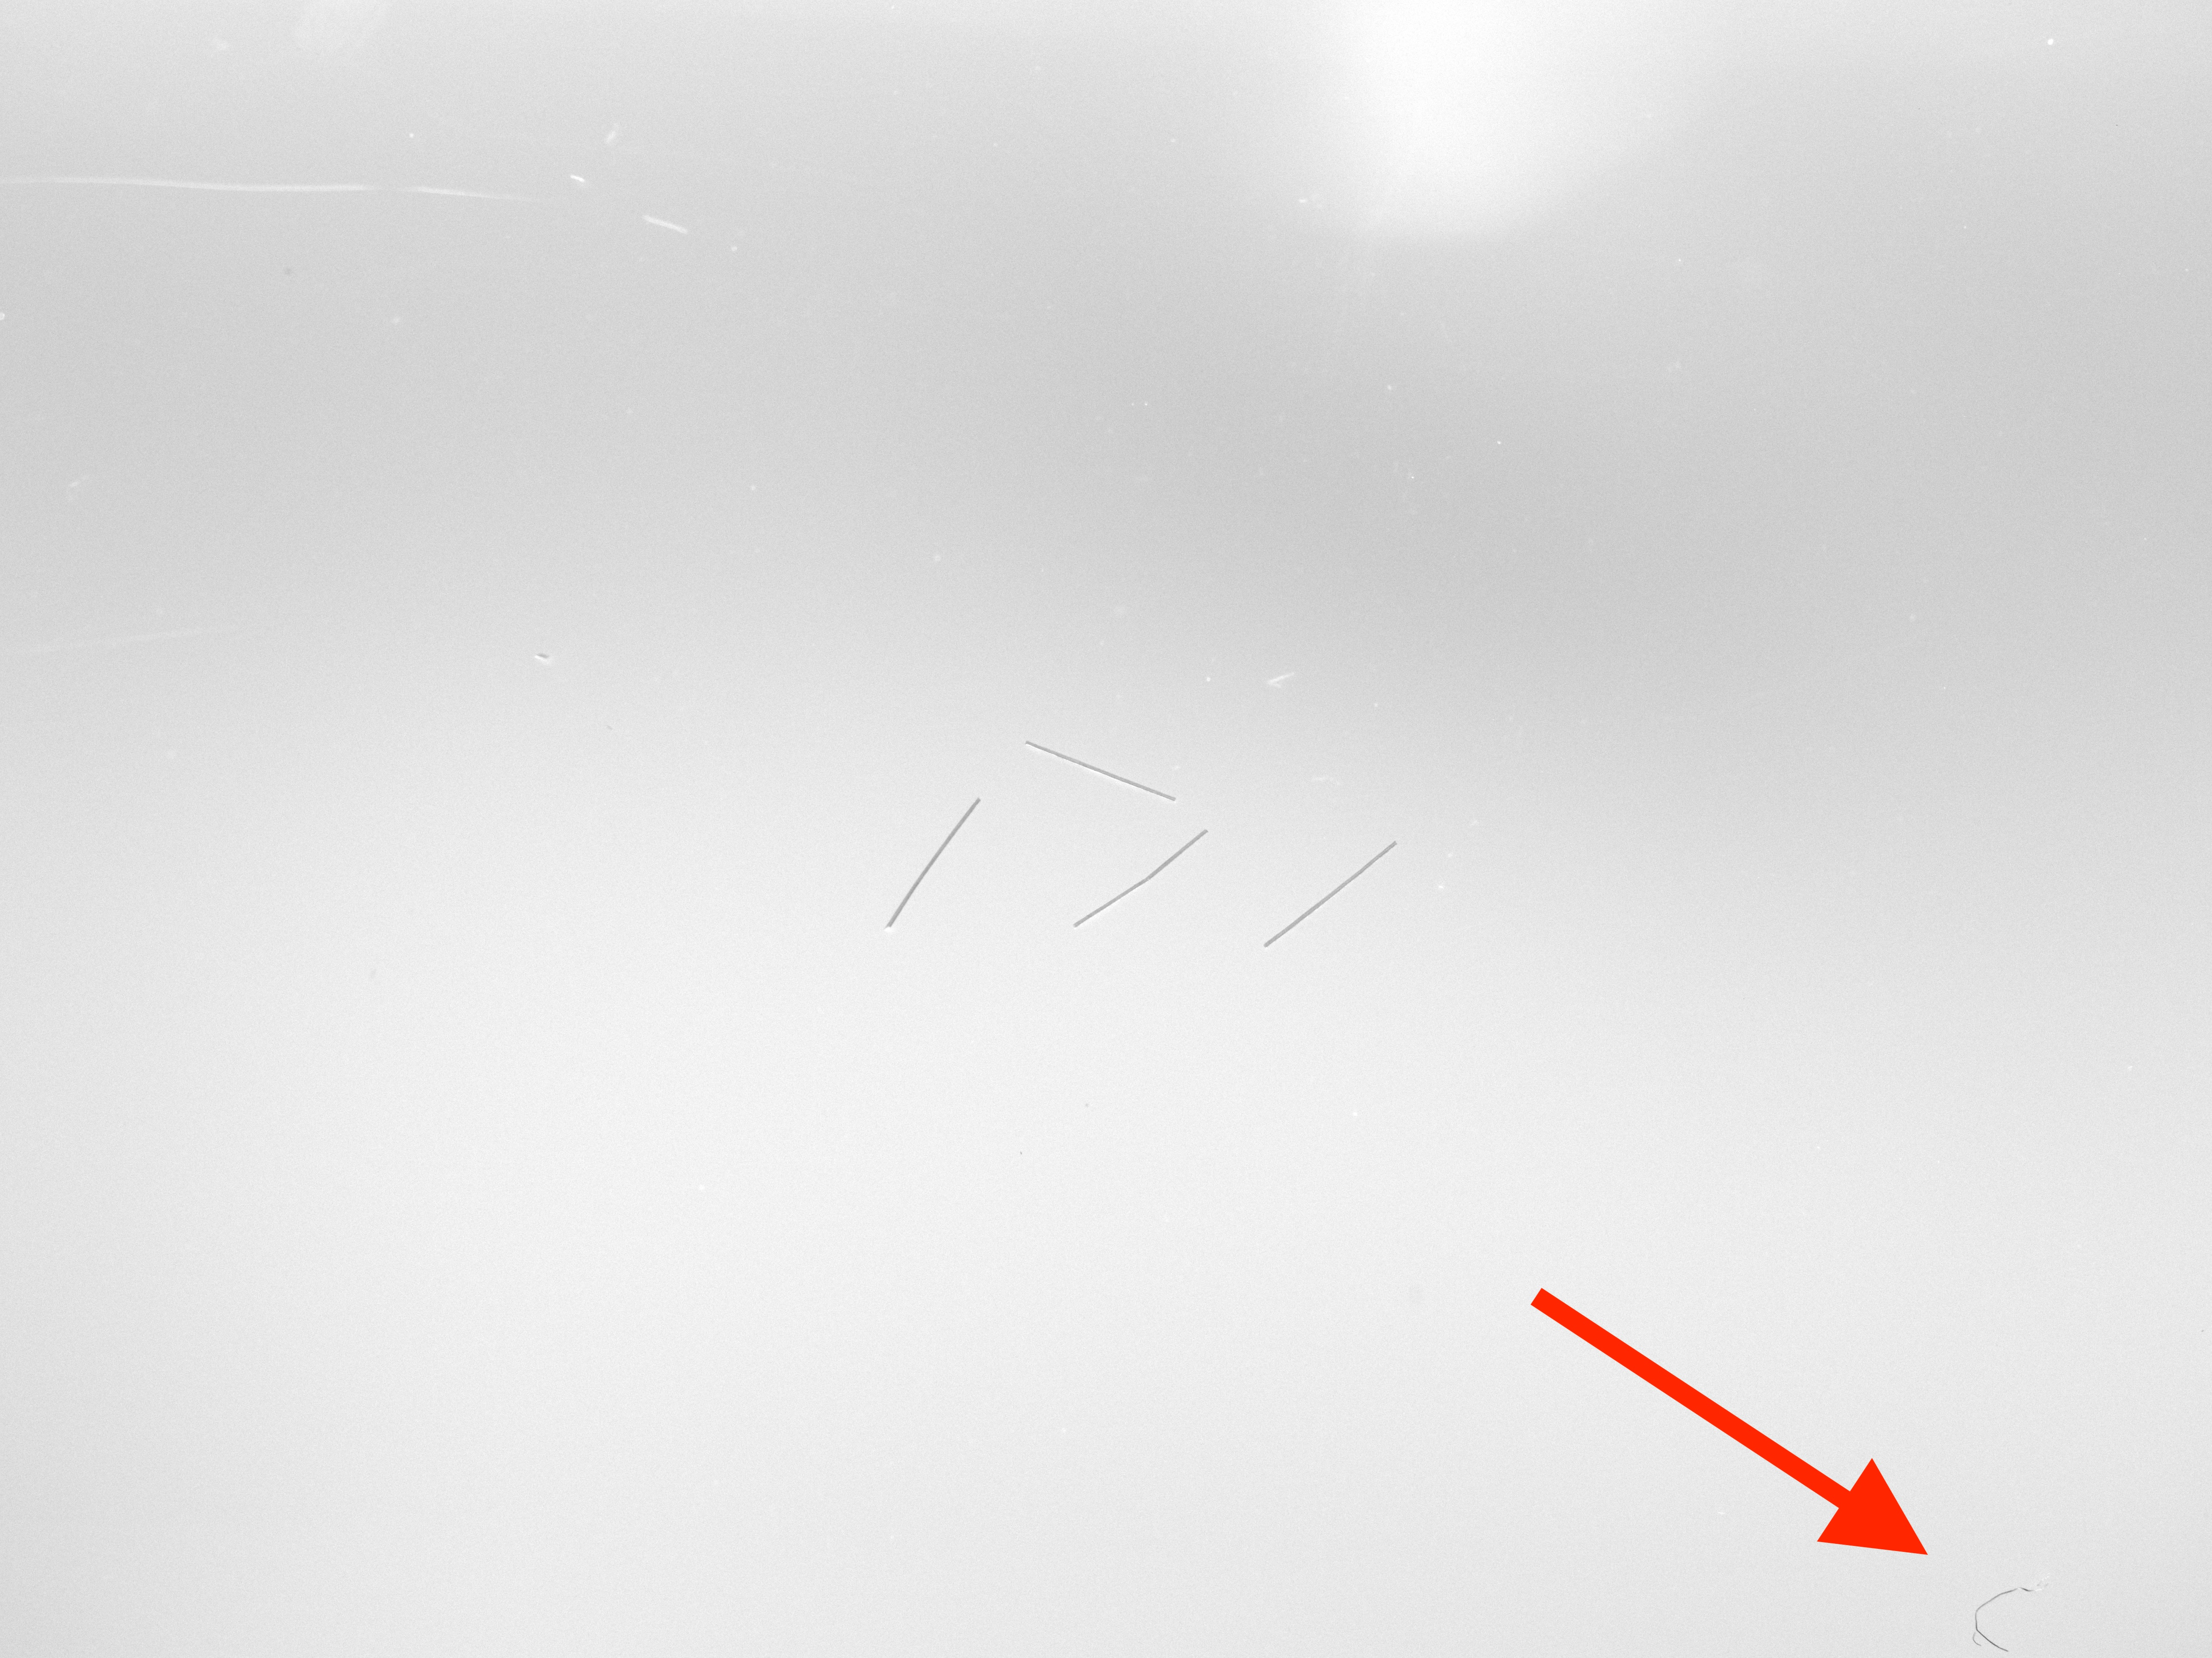
\includegraphics[width=1\linewidth]{../docs/assets/artefact} \caption{Image of hair sample with artefact biasing the measurement}\label{fig:artefact_im}
\end{figure}

The red arrow points to a stray fiber that likely contaminated the
sample and was missed during imaging. Such potential outliers are the
reason we chose to use the median curvature for a sample in our
analyses.

\hypertarget{objective-hair-texture-classification-vs.-quantitative-curvature}{%
\section{Objective hair texture classification vs.~quantitative
curvature}\label{objective-hair-texture-classification-vs.-quantitative-curvature}}

To explore how much data is lost when binning continuous variation, we
compared mean and median curvature to classified hair texture. This
classification is based on Loussouarn et al.'s 2007 paper
\href{https://doi.org/10.1111/j.1365-4632.2007.03453.x}{"Worldwide
diversity of hair curliness: a new method of assessment}.

While the authors propose a number of parameters to distinguish curlier
hair types (based on number of twists and waves among other factors),
their primary classification is based on curvature. We demonstrate that,
regardless of additional parameters, a considerable range of curvature
is obscured when collapsing hair variation according to their curvature
thresholds.

\begin{figure}
\includegraphics[width=1\linewidth]{significance_files/figure-latex/plt_admixed_HairTypeBin-1} \caption{Objective hair classification vs. quantitative curvature}\label{fig:plt_admixed_HairTypeBin}
\end{figure}

\hypertarget{ancestry-vs.-hair-morphology}{%
\section{Ancestry vs.~hair
morphology}\label{ancestry-vs.-hair-morphology}}

We carried out a number of analyses using the genotype data collected
for this diverse sample. In an admixed sample where a continuous trait
has divergent distributions in the parental ancestry groups, the
resulting admixed population can show a correlation between ancestry and
that trait. Finding such a correlation suggests may imply a polygenic
trait with high heritability.

\hypertarget{admixture-components}{%
\subsection{Admixture components}\label{admixture-components}}

Our sample consists of admixed individuals with primarily African and
European ancestry.

\begin{figure}
\includegraphics[width=1\linewidth]{significance_files/figure-latex/plt_admixture-1} \caption{Admixture components for sample}\label{fig:plt_admixture}
\end{figure}

The colors represent ancestries that correspond to the following 1000
Genomes populations: - SAS = South Asian - AMR = American - AFR =
African - EUR = European - EAS = East Asian

Each of these are metapopulations based on the grouping of multiple
(sub)continental population groups in the
\href{https://www.internationalgenome.org/category/population/}{1000
Genomes repository}.

\hypertarget{ancestry-vs.-curvature}{%
\subsection{Ancestry vs.~curvature}\label{ancestry-vs.-curvature}}

Here we plot the correlation between proportion of African ancestry and
m-index, median curvature, and eccentricity.

\begin{figure}
\includegraphics[width=1\linewidth]{significance_files/figure-latex/plt_anc_corr-1} \caption{Percentage of African ancestry vs. M-index, curvature and eccentricity}\label{fig:plt_anc_corr}
\end{figure}

\hypertarget{curvature-vs.-eccentricity}{%
\subsection{Curvature
vs.~eccentricity}\label{curvature-vs.-eccentricity}}

The relationship between cross-sectional shape (eccentricity) and
curvature has long been debated. Due to the coincidence of
cross-sectional shape and curvature in various populations that are
often contrasted (i.e.~East Asian vs.~North European vs.~West African),
it has been unclear whether these traits have a causal relationship
(specifically that higher eccentricity predicts higher curvature). In
our admixed sample, we have the opportunity to test this question and
fit a model between these traits with and without ancestry.

\hypertarget{uncorrected}{%
\subsubsection{Uncorrected}\label{uncorrected}}

First we examine the data without correcting for ancestry.

\begin{verbatim}
## 
## Call:
## lm(formula = curv_median ~ eccentricity_median, data = df_curv_ecc)
## 
## Residuals:
##     Min      1Q  Median      3Q     Max 
## -0.2843 -0.1245 -0.0264  0.1125  0.4770 
## 
## Coefficients:
##                     Estimate Std. Error t value Pr(>|t|)    
## (Intercept)          -0.5682     0.1270  -4.474 1.94e-05 ***
## eccentricity_median   1.0284     0.1692   6.076 1.96e-08 ***
## ---
## Signif. codes:  0 '***' 0.001 '**' 0.01 '*' 0.05 '.' 0.1 ' ' 1
## 
## Residual standard error: 0.1576 on 106 degrees of freedom
## Multiple R-squared:  0.2583, Adjusted R-squared:  0.2513 
## F-statistic: 36.92 on 1 and 106 DF,  p-value: 1.959e-08
\end{verbatim}

\begin{figure}
\includegraphics[width=1\linewidth]{significance_files/figure-latex/plt_curv_ecc-1} \caption{Curvature vs. eccentricity (without correction for ancestry)}\label{fig:plt_curv_ecc}
\end{figure}

If we consider the relationship between curvature and eccentricity
without taking into account ancestry, we find that eccentricity is a
significant predictor of curvature.

\hypertarget{corrected}{%
\subsubsection{Corrected}\label{corrected}}

We then re-analyze the data with ancestry as a covariate.

\begin{verbatim}
## 
## Call:
## lm(formula = curv_median ~ eccentricity_median + AFR, data = df_curv_ecc)
## 
## Residuals:
##      Min       1Q   Median       3Q      Max 
## -0.37902 -0.04122 -0.00657  0.03606  0.29971 
## 
## Coefficients:
##                     Estimate Std. Error t value Pr(>|t|)    
## (Intercept)         -0.07237    0.08661  -0.836    0.405    
## eccentricity_median  0.10891    0.12511   0.871    0.386    
## AFR                  0.48101    0.03632  13.243   <2e-16 ***
## ---
## Signif. codes:  0 '***' 0.001 '**' 0.01 '*' 0.05 '.' 0.1 ' ' 1
## 
## Residual standard error: 0.09693 on 105 degrees of freedom
## Multiple R-squared:  0.7222, Adjusted R-squared:  0.7169 
## F-statistic: 136.5 on 2 and 105 DF,  p-value: < 2.2e-16
\end{verbatim}

\begin{figure}
\includegraphics[width=1\linewidth]{significance_files/figure-latex/plt_curv_ecc_anc-1} \caption{Curvature vs. eccentricity (with correction for ancestry)}\label{fig:plt_curv_ecc_anc}
\end{figure}

However, when we correct for ancestry, this correlation is no longer
significant. This supports the idea that these traits may be
independent.

\hypertarget{curvature-vs.-skin-pigmentation}{%
\subsection{Curvature vs.~skin
pigmentation}\label{curvature-vs.-skin-pigmentation}}

To demonstrate the potential effect of population stratification on
traits, we compare hair curvature with skin pigmentation (m-index).
These two traits are not biologically related, yet, in an admixed
population, we may see a correlation that is due to population
stratification of these polygenic traits.

\hypertarget{uncorrected-1}{%
\subsubsection{Uncorrected}\label{uncorrected-1}}

First we examine the relationship between curvature and skin
pigmentation without correcting for ancestry.

\begin{verbatim}
## 
## Call:
## lm(formula = curv_median ~ m_index, data = df_curv_mindex)
## 
## Residuals:
##      Min       1Q   Median       3Q      Max 
## -0.20715 -0.06804 -0.03471  0.04818  0.51483 
## 
## Coefficients:
##              Estimate Std. Error t value Pr(>|t|)    
## (Intercept) -0.280232   0.041533  -6.747 4.91e-10 ***
## m_index      0.012887   0.001031  12.501  < 2e-16 ***
## ---
## Signif. codes:  0 '***' 0.001 '**' 0.01 '*' 0.05 '.' 0.1 ' ' 1
## 
## Residual standard error: 0.1261 on 126 degrees of freedom
## Multiple R-squared:  0.5536, Adjusted R-squared:  0.5501 
## F-statistic: 156.3 on 1 and 126 DF,  p-value: < 2.2e-16
\end{verbatim}

\begin{figure}
\includegraphics[width=1\linewidth]{significance_files/figure-latex/plt_curv_mindex-1} \caption{Curvature vs. M-index (without correction for ancestry)}\label{fig:plt_curv_mindex}
\end{figure}

As expected, we see a significant correlation between the two traits.

\hypertarget{corrected-1}{%
\subsubsection{Corrected}\label{corrected-1}}

We then apply a correction for ancestry and re-analyze the data.

\begin{verbatim}
## 
## Call:
## lm(formula = curv_median ~ m_index + AFR, data = df_curv_mindex)
## 
## Residuals:
##      Min       1Q   Median       3Q      Max 
## -0.34321 -0.04877 -0.01348  0.03562  0.34806 
## 
## Coefficients:
##              Estimate Std. Error t value Pr(>|t|)    
## (Intercept) -0.061501   0.042384  -1.451    0.149    
## m_index      0.002734   0.001469   1.862    0.065 .  
## AFR          0.406609   0.048561   8.373 9.63e-14 ***
## ---
## Signif. codes:  0 '***' 0.001 '**' 0.01 '*' 0.05 '.' 0.1 ' ' 1
## 
## Residual standard error: 0.1014 on 125 degrees of freedom
## Multiple R-squared:  0.714,  Adjusted R-squared:  0.7094 
## F-statistic:   156 on 2 and 125 DF,  p-value: < 2.2e-16
\end{verbatim}

\begin{figure}
\includegraphics[width=1\linewidth]{significance_files/figure-latex/plt_curv_mindex_anc-1} \caption{Curvature vs. M-index (with correction for ancestry)}\label{fig:plt_curv_mindex_anc}
\end{figure}

Like with curvature and eccentricity, the relationship between curvature
and skin pigmentation is no longer significant when ancestry is taken
into account.

\end{document}
